\documentclass[14pt]{extbook}
\usepackage{multicol, enumerate, enumitem, hyperref, color, soul, setspace, parskip, fancyhdr} %General Packages
\usepackage{amssymb, amsthm, amsmath, latexsym, units, mathtools} %Math Packages
\everymath{\displaystyle} %All math in Display Style
% Packages with additional options
\usepackage[headsep=0.5cm,headheight=12pt, left=1 in,right= 1 in,top= 1 in,bottom= 1 in]{geometry}
\usepackage[usenames,dvipsnames]{xcolor}
\usepackage{dashrule}  % Package to use the command below to create lines between items
\newcommand{\litem}[1]{\item#1\hspace*{-1cm}\rule{\textwidth}{0.4pt}}
\pagestyle{fancy}
\lhead{Makeup Progress Quiz 2}
\chead{}
\rhead{Version A}
\lfoot{2790-1423}
\cfoot{}
\rfoot{Summer C 2021}
\begin{document}

\begin{enumerate}
\litem{
Which of the following equations \textit{could} be of the graph presented below?
\begin{center}
    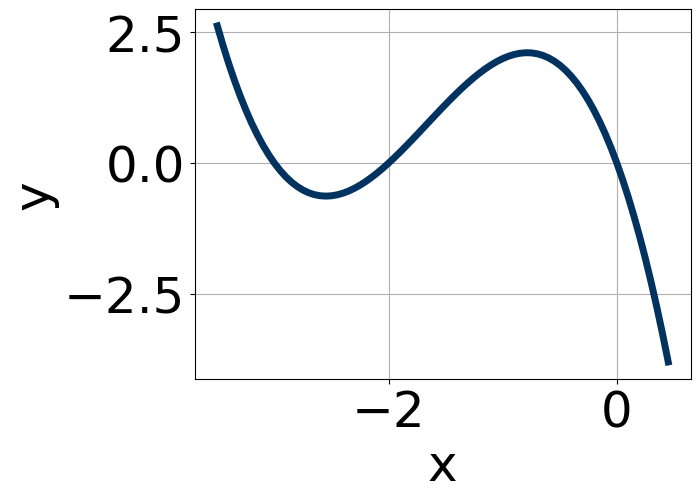
\includegraphics[width=0.5\textwidth]{../Figures/polyGraphToFunctionA.png}
\end{center}
\begin{enumerate}[label=\Alph*.]
\item \( -19x^{11} (x + 2)^{9} (x + 3)^{9} \)
\item \( 8x^{7} (x + 2)^{11} (x + 3)^{9} \)
\item \( -2x^{9} (x + 2)^{10} (x + 3)^{8} \)
\item \( -19x^{5} (x + 2)^{8} (x + 3)^{9} \)
\item \( 15x^{9} (x + 2)^{6} (x + 3)^{7} \)

\end{enumerate} }
\litem{
Construct the lowest-degree polynomial given the zeros below. Then, choose the intervals that contain the coefficients of the polynomial in the form $ax^3+bx^2+cx+d$.\[ \frac{-3}{2}, -7, \text{ and } \frac{7}{2} \]\begin{enumerate}[label=\Alph*.]
\item \( a \in [1, 7], b \in [20, 23], c \in [-77, -71], \text{ and } d \in [-149, -143] \)
\item \( a \in [1, 7], b \in [-20, -13], c \in [-77, -71], \text{ and } d \in [147, 150] \)
\item \( a \in [1, 7], b \in [6, 15], c \in [-120, -118], \text{ and } d \in [147, 150] \)
\item \( a \in [1, 7], b \in [20, 23], c \in [-77, -71], \text{ and } d \in [147, 150] \)
\item \( a \in [1, 7], b \in [-52, -47], c \in [158, 164], \text{ and } d \in [-149, -143] \)

\end{enumerate} }
\litem{
Describe the zero behavior of the zero $x = -7$ of the polynomial below.\[ f(x) = -2(x - 4)^{8}(x + 4)^{5}(x + 7)^{10}(x - 7)^{9} \]\begin{enumerate}[label=\Alph*.]
\begin{multicols}{2}\item 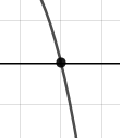
\includegraphics[width = 0.3\textwidth]{../Figures/polyZeroBehaviorCopyAA.png}\item 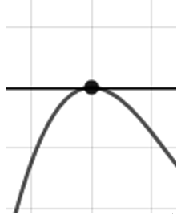
\includegraphics[width = 0.3\textwidth]{../Figures/polyZeroBehaviorCopyBA.png}\item 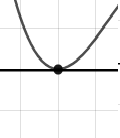
\includegraphics[width = 0.3\textwidth]{../Figures/polyZeroBehaviorCopyCA.png}\item 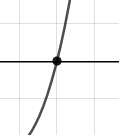
\includegraphics[width = 0.3\textwidth]{../Figures/polyZeroBehaviorCopyDA.png}\end{multicols}\item None of the above.
\end{enumerate} }
\litem{
Describe the end behavior of the polynomial below.\[ f(x) = 7(x - 7)^{2}(x + 7)^{3}(x - 8)^{5}(x + 8)^{5} \]\begin{enumerate}[label=\Alph*.]
\begin{multicols}{2}\item 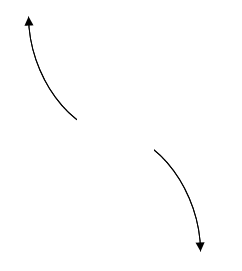
\includegraphics[width = 0.3\textwidth]{../Figures/polyEndBehaviorCopyAA.png}\item 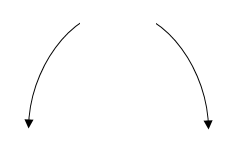
\includegraphics[width = 0.3\textwidth]{../Figures/polyEndBehaviorCopyBA.png}\item 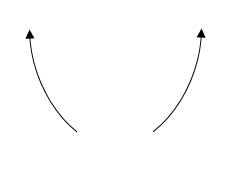
\includegraphics[width = 0.3\textwidth]{../Figures/polyEndBehaviorCopyCA.png}\item 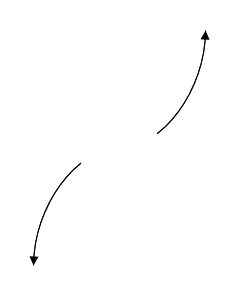
\includegraphics[width = 0.3\textwidth]{../Figures/polyEndBehaviorCopyDA.png}\end{multicols}\item None of the above.
\end{enumerate} }
\litem{
Describe the end behavior of the polynomial below.\[ f(x) = 2(x - 2)^{4}(x + 2)^{7}(x - 4)^{2}(x + 4)^{2} \]\begin{enumerate}[label=\Alph*.]
\begin{multicols}{2}\item 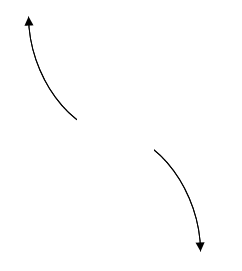
\includegraphics[width = 0.3\textwidth]{../Figures/polyEndBehaviorAA.png}\item 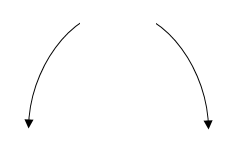
\includegraphics[width = 0.3\textwidth]{../Figures/polyEndBehaviorBA.png}\item 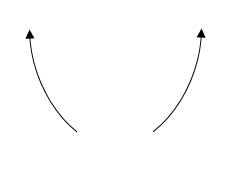
\includegraphics[width = 0.3\textwidth]{../Figures/polyEndBehaviorCA.png}\item 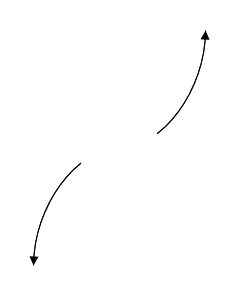
\includegraphics[width = 0.3\textwidth]{../Figures/polyEndBehaviorDA.png}\end{multicols}\item None of the above.
\end{enumerate} }
\litem{
Construct the lowest-degree polynomial given the zeros below. Then, choose the intervals that contain the coefficients of the polynomial in the form $x^3+bx^2+cx+d$.\[ -4 + 4 i \text{ and } 4 \]\begin{enumerate}[label=\Alph*.]
\item \( b \in [0.9, 3.2], c \in [-3, 3], \text{ and } d \in [-18, -14] \)
\item \( b \in [0.9, 3.2], c \in [-10, -7], \text{ and } d \in [13, 21] \)
\item \( b \in [-7.8, -3.9], c \in [-3, 3], \text{ and } d \in [121, 134] \)
\item \( b \in [3.1, 5.5], c \in [-3, 3], \text{ and } d \in [-130, -123] \)
\item \( \text{None of the above.} \)

\end{enumerate} }
\litem{
Construct the lowest-degree polynomial given the zeros below. Then, choose the intervals that contain the coefficients of the polynomial in the form $ax^3+bx^2+cx+d$.\[ -3, \frac{-5}{2}, \text{ and } \frac{-1}{5} \]\begin{enumerate}[label=\Alph*.]
\item \( a \in [10, 15], b \in [51, 61], c \in [80, 87], \text{ and } d \in [11, 19] \)
\item \( a \in [10, 15], b \in [-53, -46], c \in [53, 71], \text{ and } d \in [11, 19] \)
\item \( a \in [10, 15], b \in [-57, -54], c \in [80, 87], \text{ and } d \in [-17, -7] \)
\item \( a \in [10, 15], b \in [-3, 6], c \in [-81, -75], \text{ and } d \in [-17, -7] \)
\item \( a \in [10, 15], b \in [51, 61], c \in [80, 87], \text{ and } d \in [-17, -7] \)

\end{enumerate} }
\litem{
Which of the following equations \textit{could} be of the graph presented below?
\begin{center}
    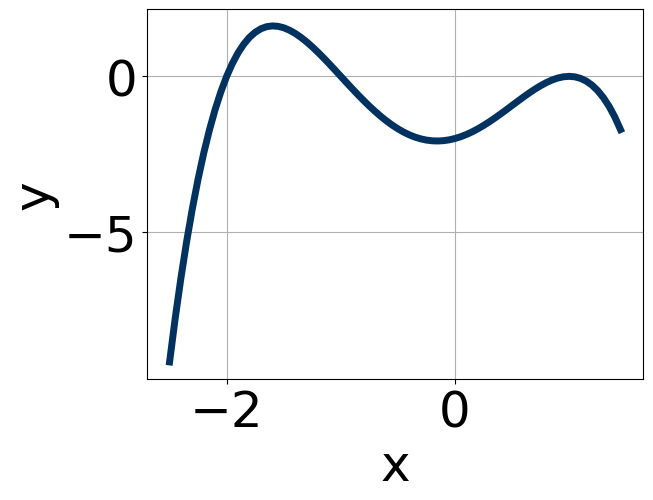
\includegraphics[width=0.5\textwidth]{../Figures/polyGraphToFunctionCopyA.png}
\end{center}
\begin{enumerate}[label=\Alph*.]
\item \( -15(x - 1)^{8} (x + 1)^{11} (x + 2)^{7} \)
\item \( -11(x - 1)^{8} (x + 1)^{6} (x + 2)^{9} \)
\item \( 16(x - 1)^{8} (x + 1)^{9} (x + 2)^{11} \)
\item \( -14(x - 1)^{7} (x + 1)^{8} (x + 2)^{9} \)
\item \( 11(x - 1)^{4} (x + 1)^{11} (x + 2)^{4} \)

\end{enumerate} }
\litem{
Construct the lowest-degree polynomial given the zeros below. Then, choose the intervals that contain the coefficients of the polynomial in the form $x^3+bx^2+cx+d$.\[ -3 - 4 i \text{ and } -2 \]\begin{enumerate}[label=\Alph*.]
\item \( b \in [-1, 5], c \in [1.8, 5.3], \text{ and } d \in [5.8, 6.4] \)
\item \( b \in [-1, 5], c \in [5.2, 8.8], \text{ and } d \in [7.7, 10.7] \)
\item \( b \in [4, 9], c \in [35.8, 38.9], \text{ and } d \in [46.8, 52.1] \)
\item \( b \in [-9, -3], c \in [35.8, 38.9], \text{ and } d \in [-50.4, -49] \)
\item \( \text{None of the above.} \)

\end{enumerate} }
\litem{
Describe the zero behavior of the zero $x = -8$ of the polynomial below.\[ f(x) = -2(x - 8)^{8}(x + 8)^{11}(x + 9)^{9}(x - 9)^{13} \]\begin{enumerate}[label=\Alph*.]
\begin{multicols}{2}\item 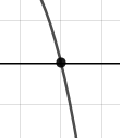
\includegraphics[width = 0.3\textwidth]{../Figures/polyZeroBehaviorAA.png}\item 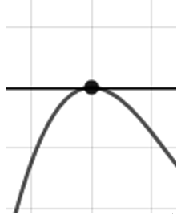
\includegraphics[width = 0.3\textwidth]{../Figures/polyZeroBehaviorBA.png}\item 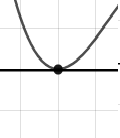
\includegraphics[width = 0.3\textwidth]{../Figures/polyZeroBehaviorCA.png}\item 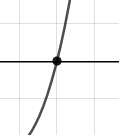
\includegraphics[width = 0.3\textwidth]{../Figures/polyZeroBehaviorDA.png}\end{multicols}\item None of the above.
\end{enumerate} }
\end{enumerate}

\end{document}